%% LyX 1.6.4 created this file.  For more info, see http://www.lyx.org/.
%% Do not edit unless you really know what you are doing.
\documentclass[english,20pt,dvips]{foils}
\usepackage[latin9]{inputenc}
\usepackage{geometry}
\geometry{verbose}
\usepackage{color}
\usepackage{pifont}
\usepackage{url}
\usepackage{amsmath}
\usepackage{graphicx}
\usepackage{amssymb}

\makeatletter

%%%%%%%%%%%%%%%%%%%%%%%%%%%%%% LyX specific LaTeX commands.
%% Because html converters don't know tabularnewline
\providecommand{\tabularnewline}{\\}
%% A simple dot to overcome graphicx limitations
\newcommand{\lyxdot}{.}


%%%%%%%%%%%%%%%%%%%%%%%%%%%%%% User specified LaTeX commands.
\newcommand{\answer}[2]{#1}

\AtBeginDocument{
  \def\labelitemi{\ding{122}}
  \def\labelitemii{\ding{229}}
}

\makeatother

\usepackage{babel}

\begin{document}
\selectlanguage{english}

\leftheader{Neil Lawrence}


\rightheader{Network Performance Analysis}


\MyLogo{\includegraphics[scale=0.4]{/home/neil/tex/inputs/sheffieldlogo}}


\rightfooter{\includegraphics[scale=1.4]{/home/neil/tex/inputs/dcslogo}\quad \thepage{}}


\title{Network Performance Analysis}


\author{Neil Lawrence}


\date{Autumn Term 2005-2006}

\maketitle

\foilhead[-0.5in]{Schedule}

Lectures will take place in the following locations:
\begin{description}
\item [{Mondays}] 15:10 - 17:00 pm (St Georges LT1). 
\item [{Tuesdays}] 16:10 pm - 17:00 pm (St Georges LT22). 
\item [{Lab~Classes}] In the Lewin Lab (Monday Weeks 3 and 9).
\end{description}
\begin{center}
\small \begin{tabular}{|l|l|l|}
\multicolumn{3}{c}{\textbf{Week 1}}\tabularnewline
\hline 
Monday & Lectures 1 \& 2 & Probability Review and Poisson Processes\tabularnewline
\hline 
Tuesday & Lecture 3 & Birth Death Processes\tabularnewline
\hline 
\multicolumn{3}{c}{\textbf{Week 2}}\tabularnewline
\hline 
Monday & Lecture 3 \& 4 & $M/M/1$ queues and Little's Formula\tabularnewline
\hline 
Tuesday & Tutorial 1 & Probability and Poisson Processes\tabularnewline
\hline 
\multicolumn{3}{c}{\textbf{Week 3}}\tabularnewline
\hline 
Monday & Lab Class 1 & Discrete Simulation of the $M/M/1$ Queue\tabularnewline
\hline 
Tuesday & Lecture 6 & Other Markov Queues\tabularnewline
\hline 
\multicolumn{3}{c}{\textbf{Week 4}}\tabularnewline
\hline 
Monday & Lectures 7 \& 8 & Erlang Delay and Erlang Loss\tabularnewline
\hline 
Tuesday & Lab Review 1 & Review of Lab Class 1\tabularnewline
\hline 
\multicolumn{3}{c}{\textbf{Week 5}}\tabularnewline
\hline 
Monday & Lectures 9 \& 10 & Erlang Loss and Markov Queues Review\tabularnewline
\hline 
Tuesday & Tutorial 2 & $M/M/1$ and Little's Formula\tabularnewline
\hline 
\multicolumn{3}{c}{\textbf{Week 6}}\tabularnewline
\hline 
\multicolumn{3}{|c|}{No Scheduled Lectures}\tabularnewline
\hline 
\multicolumn{3}{c}{\textbf{Week 7}}\tabularnewline
\hline 
Monday & Lectures 11 \& 12 & $M/G/1$ and $M/G/1$ with Vacations\tabularnewline
\hline 
Tuesday & Lecture 13 & $M/G/1$ contd\tabularnewline
\hline 
\multicolumn{3}{c}{\textbf{Week 8}}\tabularnewline
\hline 
Monday & Lectures 14 \& 15 & Networks of Queues\tabularnewline
\hline 
Tuesday & Tutorial 3 & Erlang Delay and Loss, $M/G/1$\tabularnewline
\hline 
\multicolumn{3}{c}{\textbf{Week 9}}\tabularnewline
\hline 
Monday & Lab Class 2 & Simulation of Queues in NS2\tabularnewline
\hline 
Tuesday & Lecture 16 & Jackson's Theorem\tabularnewline
\hline 
\multicolumn{3}{c}{\textbf{Week 10}}\tabularnewline
\hline 
Tuesday & Lab Review 2 & Review of NS2 Lab Class\tabularnewline
\hline 
\multicolumn{3}{c}{\textbf{Week 11}}\tabularnewline
\hline 
\multicolumn{3}{|c|}{No Scheduled Lectures}\tabularnewline
\hline 
\multicolumn{3}{c}{\textbf{Week 12}}\tabularnewline
\hline 
\multicolumn{3}{|c|}{No Scheduled Lectures}\tabularnewline
\hline 
\multicolumn{3}{c}{\textbf{Week 13 (tentative)}}\tabularnewline
\hline 
Monday & Past Paper Review & Review of the 2004-05 Exam Paper\tabularnewline
\hline
\end{tabular}\normalsize 
\par\end{center}
\begin{itemize}
\item \textbf{Evaluation}: This course is 100\% exam. 
\end{itemize}

\foilhead[-0.5in]{Reading List}

The course is based primarily on \cite{Bertsekas:data92}. The relevant
parts of the book are as follows. 
\begin{description}
\item [{Chapter~1}] For background reading and review. 
\item [{Chapter~3}] Section 3.1 -- 3.5 For queueing models. 
\item [{Chapter~4}] In less detail: Section 4.1 -- 4.4, Section 4.5.2,
4.5.3. 
\end{description}
For additional background reading you may wish to consult some of
the books listed below, \cite{Tanenbaum:computer96} is the standard
text for Introductory courses, but has little coverage on queueing
theory. \cite{Chan:performance00} is an alternative text for details
on queues.

There is additional material on-line at the course web-site: \url{http://www.dcs.shef.ac.uk/~neil/campus_only/com6131/}.


\foilhead[-0.5in]{Your Notes}
\begin{itemize}
\item Designed to accompany \cite{Bertsekas:data92}, cover in extra detail
areas of importance for the course and adding material where it is
lacking (for example on simulation).
\item First three chapters provide background material on networks and probabilities.
\item Please inform me of any errors in these notes using the form provided
on the course website.
\end{itemize}

\foilhead[-0.5in]{Introduction and Background}


\foilhead[-0.5in]{Introduction}
\begin{itemize}
\item Queueing theory dates back to the beginning of the 20th Century and
the pioneering work of Agner Krarup Erlang (1878-1929).
\item Erlang was a Danish Telecoms Engineer who published the first paper
on queueing theory \cite{Erlang:theory09}.
\item Initially, telephone call routing was achieved manually. 
\item The invention of the \emph{automatic telephone exchange} (through
the Strowger switch) in 1891 brought about the need for a theoretical
study of the operation of telephone exchanges.
\item Erlang's provided theoretical studies of these circuit switching networks.
\end{itemize}

\foilhead[-0.5in]{Computer Networks}
\begin{itemize}
\item Circuit switched networks were designed for telephone communication
between two correspondents. 
\item By the early 1960s \emph{packet switching networks} came into being.
\item ARPANET was predecessor of the internet.


%
\begin{figure}[ht]
\begin{centering}
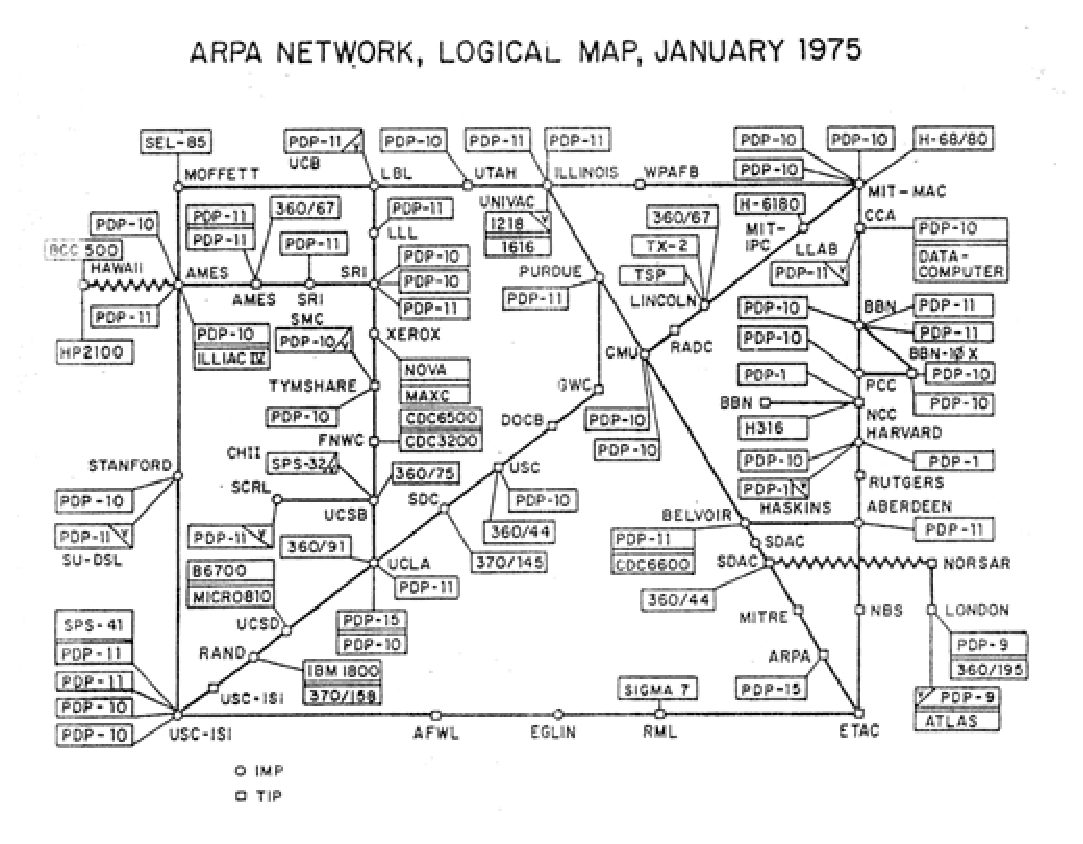
\includegraphics[scale=0.75]{diagrams/1975_net_map}
\par\end{centering}

\caption{The ARPANET in 1975, image courtesy of the Computer History Museum,
\protect\url{http://www.computerhistory.org}. }

\end{figure}


\end{itemize}

\foilhead[-0.5in]{Network Performance Analysis}
\begin{itemize}
\item In this course we will introduce you to the tools for design and analysis
of telecommunications networks. 
\item The core tools of this analysis are probability based: there is an
assumption that the traffic in the system is stochastic.
\item The techniques we will cover are applicable beyond the design and
analysis of telecommunication networks. \emph{e.g.} compute servers
dealing with submitted jobs and databases handling queries, cashpoints
queues, supermarket queues, telephone call centres \emph{etc}.. 
\end{itemize}

\foilhead[-0.5in]{Practical Considerations}

Broadly speaking we need to focus on two interrelated areas in our
analysis:
\begin{enumerate}
\item \textbf{Design Issues}: when building or buying a router how much
memory should we allow for? How much bandwidth do we need between
routers? How much processing power should the router have so that
it may exploit that bandwidth effectively?
\item \textbf{Quality Issues}: what will be the average delay for end users
given our network design? What is the worst case delay? How likely
is the system to drop packets?
\end{enumerate}
These are important because resources are finite, there are limitations
on the available bandwidth, processor speeds and memory. 


\foilhead[-0.5in]{Terminology}
\begin{itemize}
\item A series of communications between two users/computers is known as
a \emph{session}.
\item The interactions themselves consist of \emph{messages} each of which
may be split into \emph{packets}. 
\end{itemize}

\foilhead[-0.5in]{Session Characteristics}
\begin{itemize}
\item Characteristics of the session vary according to protocol:

\begin{enumerate}
\item \textbf{Message arrival rate}. We can seek to model the arrivals as:
\emph{Poisson arrivals}, \emph{deterministic arrivals}, \emph{uniform
arrivals} or as coming from a more general class of distributions.
\item \textbf{Session holding time}: The length of a session.
\item \textbf{Expected message length} and \textbf{length distribution},
message lengths can be modeled as \emph{exponential distributions},
\emph{uniform length}.
\item \textbf{Allowable delay} - acceptable expected delays vary. The acceptable
delay is low for VoIP and quite high for FTP. 
\item \textbf{Reliability} - FTP \emph{must} be error free but VoIP can
have some bit errors or packet loss without major consequences.
\item \textbf{Message and packet ordering} - Some sessions will require
that the packets arrive in the order they are sent: for example database
requests.
\end{enumerate}
\item In this course we will be particularly interested in the first five
of these characteristics. 
\end{itemize}

\foilhead[-0.5in]{Network Types}
\begin{description}
\item [{Circuit~Switching:}] used for telephone routing. Guarantees an
open `channel' between two peers. 
\item [{Packet~Switching}] or Store and Forward Switching: used for data.
May operate via 

\begin{description}
\item [{Dynamic~Routing}] Each packet of the message moves through the
network independently. 
\item [{Virtual~Circuit~Routing}] A fixed path through the network is
provided for the entire message. 
\end{description}
\end{description}
The character of the two approaches are quite different.


\foilhead[-0.5in]{Circuit~Switching}
\begin{itemize}
\item wasteful in terms of bandwidth. Nodes may not be using all the available
bandwidth reserved for them.
\item a guaranteed channel is provided with a known communication delay
associated with it.
\item the sum of rates for all sessions using a link cannot exceed the total
capacity of the link. New sessions must be rejected when the link
capacity is reached. 
\item used for telephone networks where the session rate, $r_{s}$, is the
same for each session. Switching would be more complex for data networks
and the nature of transmission would also mean that the links are
inefficiently used. 
\end{itemize}

\foilhead[-0.5in]{Packet Switching}
\begin{itemize}
\item Packet switching makes efficient use of bandwidth because, whilst
communication between two nodes may be idle for a period of time,
packets from another communication may be sent along the same line.
\item Because it is unknown \emph{a priori} how much bandwidth will be available
it is difficult to guarantee a maximum delay. 
\end{itemize}

\foilhead[-0.5in]{Communication Media}
\begin{itemize}
\item Circuit switching networks may share a communication through multiplexing
(\emph{e.g.} time division multiplexing or frequency division multiplexing.) 
\item Both are not 100\% efficient (time multiplexing requires a small amount
of time for switching to occur, and frequency division multiplexing
requires a small `buffer' band of frequencies between each session. 
\item Packet switching networks dedicate communication bandwidth to each
channel as required. In a simple `first in, first out'%
\footnote{Also known as `first come, first served' (FCFS).%
} (FIFO) system, packets arrive and, if the queue is empty, they are
transmitted. Otherwise they are stored and await their turn for transmission. 
\item In packet switching there are two delays: a queueing delay and a transmission
delay. The queueing delay is variable, transmission delay will be
fixed .
\end{itemize}

\foilhead[-0.5in]{The Road Ahead}
\begin{description}
\item [{Probability~Review}] Review of probability theory. 
\item [{Simple~Queuing~models}] Simple models of queues based on probability
theory. Little's formula, $M/M/1$ queue, $M/M/\infty$, $M/M/m$,
$M/M/m/m$ and $M/G/1$. 
\item [{Simulation}] Simulation of queueing systems.
\end{description}

\foilhead[-0.5in]{Examples}
\begin{enumerate}
\item As a simple example let's consider a database (perhaps MySQL). We
are constructing it from existing parts. We have two CPU/motherboard
systems and two separate disk systems, their expected characteristics
are shown in Table~\ref{cap:SQLserver}. Which should we match with
which? Are we better off building one faster system and one slower
system? Or should we build two systems that have a similar performance?




%
\begin{table}[ht]
\begin{centering}
\begin{tabular}{|c|c|c|c|}
\hline 
CPU  & Service Time/ms & Disk & Service Time/ms\tabularnewline
\hline
\hline 
A & 423 & 1 & 215\tabularnewline
\hline 
B & 210 & 2 & 390\tabularnewline
\hline
\end{tabular}
\par\end{centering}

\caption{Average times for a fictional database server for three different
cases.\label{cap:SQLserver}}

\end{table}


\end{enumerate}

\foilhead[-0.5in]{Probability Review}
\begin{itemize}
\item Health warning: Mathematics and Probability are FUNDAMENTAL to this
course. 
\item We are interested in trials which result in two random variables,
$X$ and $Y$, each of which has an `outcome' denoted by $x$ or $y$. 
\item We summarise the notation and terminology for these distributions
in the following table.
\end{itemize}
\begin{center}
%
\begin{table}[ht]
\begin{centering}
\small \begin{tabular}{|c|c|c|}
\hline 
Terminology & Notation & Description\tabularnewline
\hline
\hline 
Joint  & $P\left(X=x,Y=y\right)$ & `The probability that\tabularnewline
Probability &  &  $X=x$ and $Y=y$'\tabularnewline
\hline 
Marginal  & $P\left(X=x\right)$ & `The probability that\tabularnewline
Probability &  &  $X=x$ regardless of $Y$'\tabularnewline
\hline 
Conditional  & $P\left(X=x|Y=y\right)$ & `The probability that \tabularnewline
Probability &  & $X=x$ given that $Y=y$'\tabularnewline
\hline
\end{tabular}
\par\end{centering}

\caption{The different basic probability distributions.\label{cap:basicProbabilityDistributions}}

\end{table}

\par\end{center}


\foilhead[-0.5in]{A Pictorial Definition of Probability}
\begin{itemize}
\item Here is a review of what probabilities are in a two dimensional graph.
\end{itemize}
%
\begin{figure}[ht]
\begin{centering}
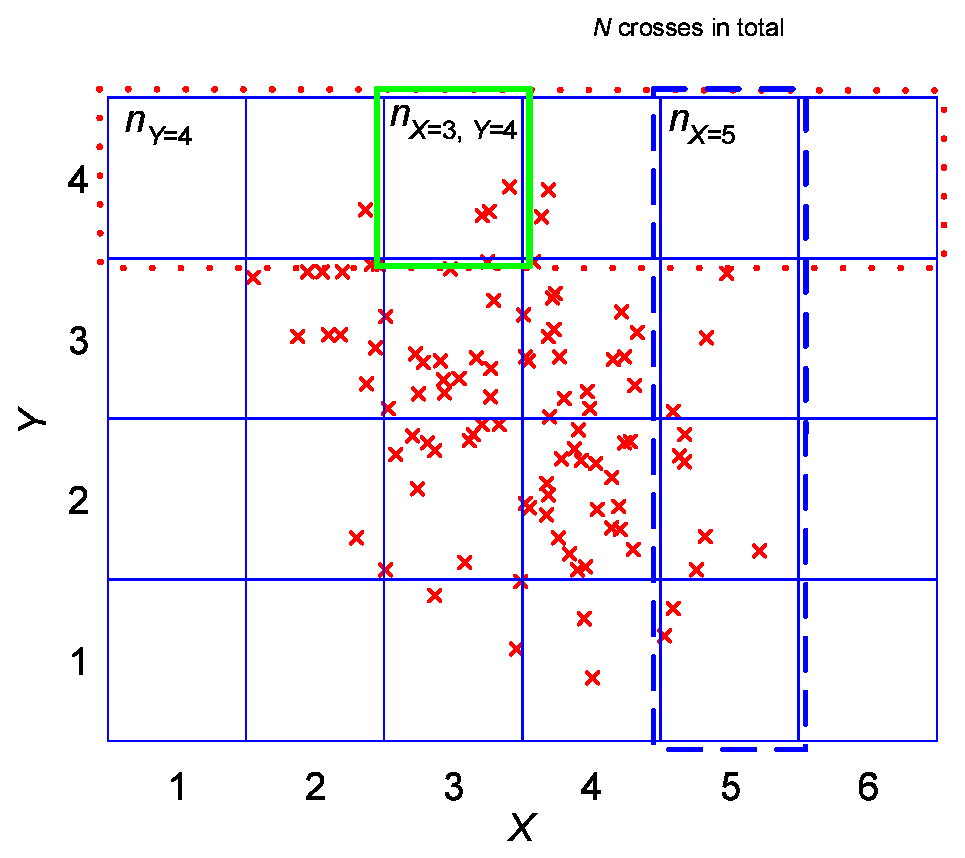
\includegraphics[width=0.8\textwidth]{diagrams/probDiagram}
\par\end{centering}

\caption{Representation of joint and conditional probabilities.\label{cap:aJointDistribution} }

\end{figure}



\foilhead[-0.5in]{Different Distributions}

%
\begin{table}[ht]
\begin{centering}
\begin{tabular}{|c|c|}
\hline 
Terminology & Definition\tabularnewline
\hline
\hline 
Joint  & $\lim_{N\rightarrow\infty}\frac{n_{X=3,Y=4}}{N}$\tabularnewline
Probability & $=P\left(X=3,Y=4\right)$\tabularnewline
\hline 
Marginal  & $\lim_{N\rightarrow\infty}\frac{n_{X=5}}{N}$\tabularnewline
Probability & $=P\left(X=5\right)$\tabularnewline
\hline 
Conditional  & $\lim_{N\rightarrow\infty}\frac{n_{X=3,Y=4}}{n_{Y=4}}$\tabularnewline
Probability & $=P\left(X=3|Y=4\right)$\tabularnewline
\hline
\end{tabular}
\par\end{centering}

\caption{Definition of probability distributions from Table~\ref{cap:basicProbabilityDistributions}
in terms of the system depicted in Figure~\ref{cap:aJointDistribution}.}

\end{table}



\foilhead[-0.5in]{Notational Details}
\begin{itemize}
\item Typically we should write out $P\left(X=x,Y=y\right)$. 
\item In practice, we often use $P\left(x,y\right)$. 
\item This looks very much like we might write a multivariate function,
\emph{e.g.} $f\left(x,y\right)=\frac{x}{y}$. 

\begin{itemize}
\item For a multivariate function though, $f\left(x,y\right)\neq f\left(y,x\right)$. 
\item However $P\left(x,y\right)=P\left(y,x\right)$ because $P\left(X=x,Y=y\right)=P\left(Y=y,X=x\right)$.
\end{itemize}
\item We have denoted the probability distribution with a capital $P$. 
\item We will use capital $P$s consistently to denote discrete distributions. 
\item For continuous probability density functions, we will turn to small
letters.
\item We now consider some `rules of probability'.
\end{itemize}

\foilhead[-0.5in]{Normalisation}

All distributions are normalised. This is clear from the fact that
$\sum_{x}n_{X=x}=N$, which gives \[
\sum_{x}P\left(x\right)=\lim_{N\rightarrow\infty}\frac{\sum_{x}n_{X=x}}{N}=\lim_{N\rightarrow\infty}\frac{N}{N}=1.\]
A similar result can be derived for the marginal and conditional distributions.


\foilhead[-0.5in]{The Sum Rule }
\begin{itemize}
\item The marginal probability $P\left(y\right)$ is given by $\lim_{N\rightarrow\infty}\frac{n_{Y=y}}{N}$.
\item The joint distribution $P\left(x,y\right)$ is given by $\lim_{N\rightarrow\infty}\frac{n_{X=x,Y=y}}{N}$. 
\item $n_{Y=y}=\sum_{x}n_{X=x,Y=y}$ so\[
\lim_{N\rightarrow\infty}\frac{n_{Y=y}}{N}=\lim_{N\rightarrow\infty}\sum_{x}\frac{n_{X=x,Y=y}}{N},\]
in other words\[
P\left(y\right)=\sum_{x}P\left(x,y\right).\]
This is known as the sum rule of probability. 
\end{itemize}

\foilhead[-0.5in]{The Product Rule}
\begin{itemize}
\item $P\left(x|y\right)$ is given by $\lim_{N\rightarrow\infty}\frac{n_{X=x,Y=y}}{n_{Y=y}}$. 
\item $P\left(x,y\right)$ is given by \[
\lim_{N\rightarrow\infty}\frac{n_{X=x,Y=y}}{N}=\lim_{N\rightarrow\infty}\frac{n_{X=x,Y=y}}{n_{Y=y}}\frac{n_{Y=y}}{N}\]
or in other words\[
P\left(x,y\right)=P\left(x|y\right)P\left(y\right).\]
This is known as the product rule of probability.
\end{itemize}

\foilhead[-0.5in]{Bayes' Rule}
\begin{itemize}
\item From the product rule,\[
P\left(x,y\right)=P\left(y,x\right)=P\left(y|x\right)P\left(x\right),\]
 


so\[
P\left(x|y\right)P\left(y\right)=P\left(y|x\right)P\left(x\right)\]
which leads to Bayes' Rule, \[
P\left(x|y\right)=\frac{P\left(y|x\right)P\left(x\right)}{P\left(y\right)}.\]


\end{itemize}

\foilhead[-0.5in]{Independence}
\begin{itemize}
\item The variable $x$ is independent of $y$ if the distribution over
$x$ is not affected by the value of $y$:\[
P\left(x\right)=P\left(x|y\right),\]
the conditional distribution of $x$ given $y$ is equal to the marginal
distribution of $x$. This in turn implies that the joint distribution
factorises,\[
P\left(x,y\right)=P\left(x|y\right)P\left(y\right)=P\left(x\right)P\left(y\right),\]
and furthermore that \[
P\left(y|x\right)=P\left(y\right).\]
The factorisation of the joint distribution when variables are independent
turns out to be a very important property which makes a lot of analysis
tractable.
\end{itemize}

\foilhead[-0.5in]{Expectations\label{sec:expectations}}
\begin{itemize}
\item A probabilistic model summarises our beliefs.
\item Sometimes need to summarise the model by its expectations.
\item Expected value of $f\left(x\right)$ under $P\left(x\right)$ is \[
\left\langle f\left(x\right)\right\rangle _{P\left(x\right)}=\sum_{x}P\left(x\right)f\left(x\right).\]
Here we have introduced a particular notation for the expectation,
you will also see expectations written in the form $E\left\{ f\left(x\right)\right\} $. 
\end{itemize}

\foilhead[-0.5in]{Expectations under a Simple Distribution}
\begin{itemize}
\item Define a distribution over $x$ in Table~\ref{cap:simpleXDistribution}.


%
\begin{table}[ht]
\begin{centering}
\begin{tabular}{|c|c|c|c|}
\hline 
$x$ & 0 & 1 & 2\tabularnewline
\hline
\hline 
$P\left(x\right)$ & 0.2 & 0.5 & 0.3\tabularnewline
\hline 
$f\left(x\right)=x^{2}$ & 0 & 1 & 4\tabularnewline
\hline
\end{tabular}
\par\end{centering}

\caption{Distribution over $x$ and associated values of $f\left(x\right)$.\label{cap:simpleXDistribution}}

\end{table}
 

\item We can compute \[
\left\langle f\left(x\right)\right\rangle =\left\langle x^{2}\right\rangle =0\times0.2+1\times0.5+4\times0.3=1.7,\]
have dropped the subscript $P\left(x\right)$
\item We can also see that the expectation of $x$ is\[
\left\langle x\right\rangle =0\times0.2+1\times0.5+2\times0.3=1.1.\]

\item The expectation of $x$ is known as the first moment of the distribution
or its \emph{mean}. 
\item The expectation of $x^{2}$ is known as the second moment --- normally
used to obtain the variance. 
\item Variance: given by the difference between the second moment and the
square of the mean. It is often denoted by $\sigma^{2}$.\[
\sigma^{2}=\left\langle x^{2}\right\rangle -\left\langle x\right\rangle ^{2}.\]
For our example above the variance is given by\[
1.7-\left(1.1\right)^{2}=0.49,\]

\item Its square root is known as the standard deviation\[
\sigma=\sqrt{\left\langle x^{2}\right\rangle -\left\langle x\right\rangle ^{2}},\]
\[
\sqrt{1.7-\left(1.1\right)^{2}}=0.7.\]

\end{itemize}

\foilhead[-0.5in]{Distributions as Functions}
\begin{itemize}
\item Probability distribution with a simple table can be limiting.
\item The Poisson Distribution --- a distribution a a function
\item First published by \textbf{Sim�on Denis Poisson} (1781-1840) in 1837. 
\item Defined over the space of all non-negative integers. 
\item This set is countably infinite: impossible to summarise in a table!
\item The Poisson distribution is therefore defined as\begin{equation}
P\left(k|\mu\right)=\frac{\mu^{k}}{k!}\exp\left(-\mu\right).\label{eq:poissonDist}\end{equation}
where $k$ is any integer from $0$ to $\infty$, and $\mu$ is a
parameter of the distribution. 
\end{itemize}

\foilhead[-0.5in]{A Poisson with $\mu=2$}
\begin{itemize}
\item To work out the probability of $k$ in a Poisson $\mu=2$ we can start
filling a table.
\item The values in a table are computed from (\ref{eq:poissonDist})%
\begin{table}[ht]
\begin{centering}
\begin{tabular}{|c|c|c|c|c|}
\hline 
$k$ & 0 & 1 & 2 & $\dots$\tabularnewline
\hline
\hline 
$P\left(x\right)$ & 0.135 & 0.271 & 0.271 & $\dots$\tabularnewline
\hline
\end{tabular}
\par\end{centering}

\caption{Some values for the Poisson distribution with $\mu=2$.\label{cap:poissonTable}}

\end{table}
 
\end{itemize}

\foilhead[-0.5in]{Mean and Variance}
\begin{itemize}
\item Example 1, Chapter 3: Mean and Variance of Poisson Distribution


As we mentioned in Section~\ref{sec:expectations}, the expectations
under a distribution are important for summarising the distributions
characteristics. Expectations of distributions that take the form
of a function can also be computed. Typically we expect the resulting
expectation to be a function of the distributions parameters.



\item The variance of a Poisson is also $\mu$ --- see Tutorial 1. 
\end{itemize}

\foilhead[-0.5in]{Continuous Variables}
\begin{itemize}
\item So far discrete values of $x$ or $y$. 
\item For continuous models we introduce the \emph{probability density function}
(PDF). 
\item Discrete case: defined probability distributions over a discrete number
of states. 
\item How do we represent continuous as probability?
\item Computer science student's height:

\begin{itemize}
\item Develop a representation which could answer \emph{any} question we
chose to ask about a computer scientist's height. 
\end{itemize}
\end{itemize}

\foilhead[-0.5in]{Gaussian PDF}
\begin{itemize}
\item One example is the Gaussian: we can query the distribution by integrating
over regions of it. 
\end{itemize}
%
\begin{figure}[ht]
\begin{centering}
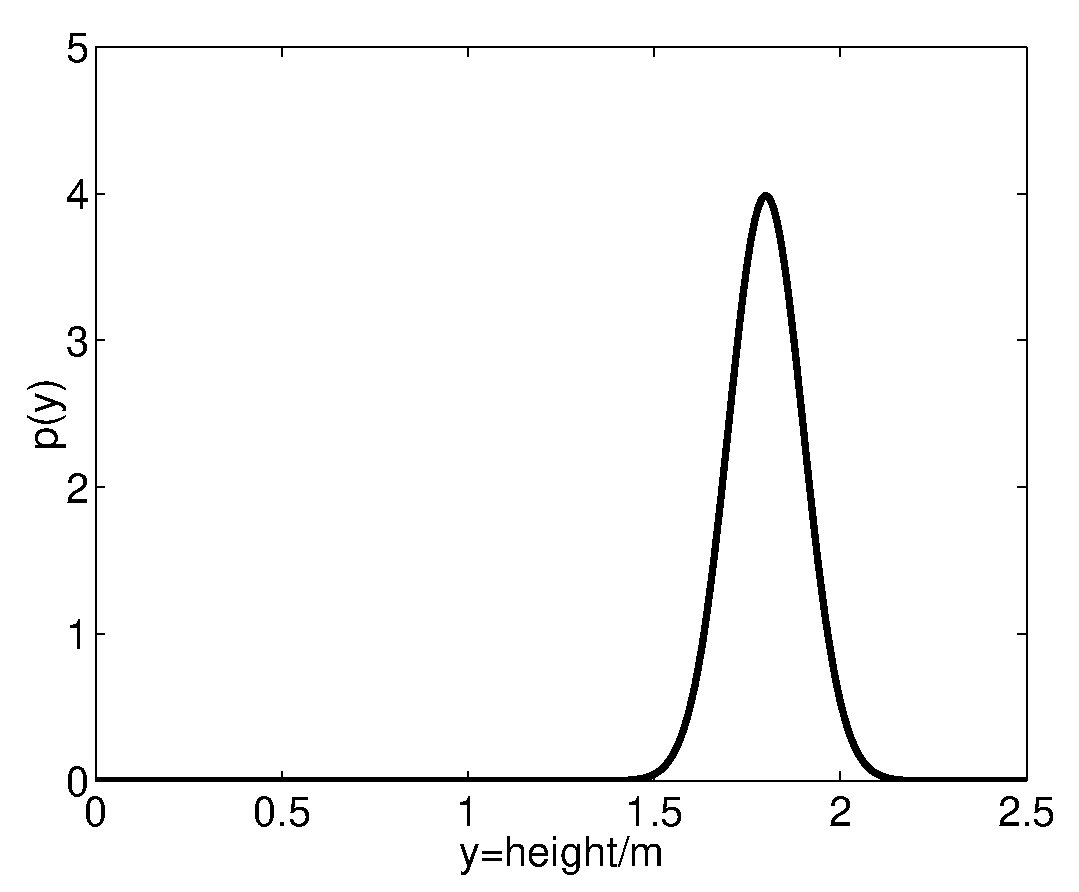
\includegraphics[scale=0.5]{diagrams/pdfOfHeight}
\par\end{centering}

\caption{A Gaussian PDF representing heights of computer scientists.\label{cap:heightPDF}}

\end{figure}

\begin{itemize}
\item Represent a PDF with a small $p\left(\cdot\right)$ to differentiate
it from a probability distribution: $P\left(\cdot\right)$. 
\item It is a positive function, integral over the region of interest is
one%
\footnote{In what follows we shall use the word distribution to refer to both
discrete probabilities and continuous probability density functions.%
}.
\end{itemize}

\foilhead[-0.5in]{Manipulating PDFs}
\begin{itemize}
\item Same rules for PDFs as distributions \emph{e.g.}\[
p\left(y|x\right)=\frac{p\left(x|y\right)p\left(y\right)}{p\left(x\right)}\]
where $p\left(x,y\right)=p\left(x|y\right)p\left(y\right)$ and for
continuous variables $p\left(x\right)=\int p\left(x,y\right)dy$. 
\item Expectations under a PDF\[
\left\langle f\left(x\right)\right\rangle _{p\left(x\right)}=\int f\left(x\right)p\left(x\right)dx\]
where the integral is over the region for which our PDF for $x$ is
defined.
\end{itemize}

\foilhead[-0.5in]{Cumulative Distribution Functions\label{sub:CDFs}}
\begin{itemize}
\item PDF doesn't represent probabilities directly
\item One very common question is: what is the probability that $x<y$? 
\item The cumulative distribution function (CDF) represents the answer for
$-\infty<x<\infty$ the CDF is given by\[
P\left(x>y\right)=\int_{-\infty}^{y}p\left(x\right)dx,\]
for $0\leq x<\infty$ then the CDF is given by\[
P\left(x>y\right)=\int_{0}^{y}p\left(x\right)dx.\]

\end{itemize}

\foilhead[-0.5in]{Gaussian PDF and CDF}
\begin{itemize}
\item In Figure~\ref{cap:heightPDF} example of the CDF for the students'
heights example.
\end{itemize}
%
\begin{figure}[ht]
\begin{centering}
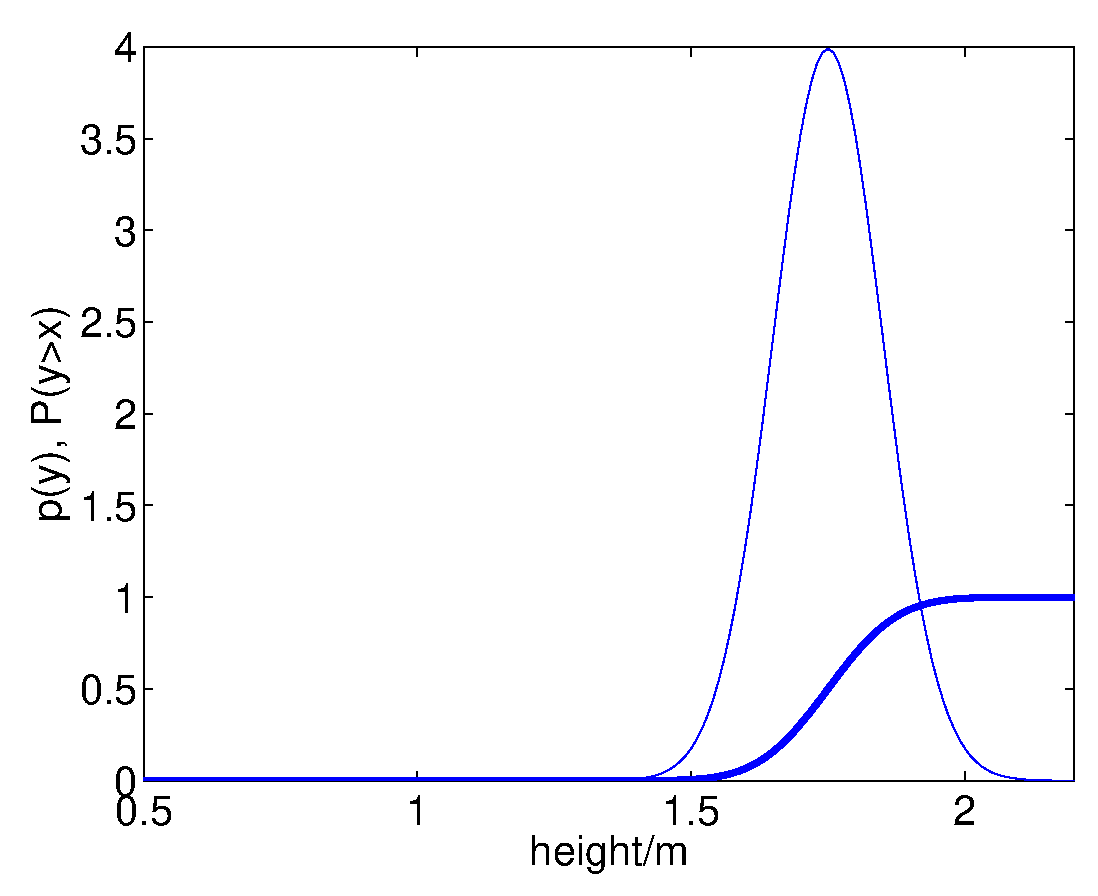
\includegraphics[scale=0.5]{diagrams/cdfOfHeight}
\par\end{centering}

\caption{The cumulative distribution function (CDF) for the heights of computer
science students. The thick curve gives the CDF and the thinner curve
the associated PDF.}

\end{figure}

\begin{itemize}
\item The PDF can be recovered from the CDF through differentiation.
\end{itemize}

\foilhead[-0.5in]{Sample Based Approximations}
\begin{itemize}
\item Recall that expectation of any given function, $f\left(k\right)$,
under a distribution, $P\left(k\right)$, can be written as \[
\left\langle f\left(k\right)\right\rangle _{P\left(k\right)}=\sum_{k}f\left(k\right)P\left(k\right)\]
Recall our definition of probability from Table~\ref{cap:aJointDistribution}.
\[
P\left(k\right)=\lim_{S\rightarrow\infty}\frac{s_{k}}{S}\]
where we have now used $S$ (instead of $N$) 
\item \emph{Sample based approximations} hope that $S$ is `large enough'
such that it to say\[
\left\langle f\left(k\right)\right\rangle _{P\left(k\right)}\approx\sum_{k}f\left(k\right)\frac{s_{k}}{S}.\]

\end{itemize}

\foilhead[-0.5in]{Sample Based Approximations contd}
\begin{itemize}
\item This formula may be rewritten as:\[
\sum_{k}f\left(k\right)\frac{s_{k}}{S}=\frac{1}{S}\sum_{k}f\left(k\right)s_{k}.\]
For $\mathbf{k}$ a vector of samples from $P\left(k\right)$with
elements $k_{i}$ and length $S$ \[
\frac{1}{S}\sum_{k}f\left(k\right)s_{k}=\frac{1}{S}\sum_{i=1}^{S}f\left(k_{i}\right)\]

\item This provides us with a sample based approximation \[
\left\langle f\left(k\right)\right\rangle _{P\left(k\right)}\approx\frac{1}{S}\sum_{i=1}^{S}f\left(k_{i}\right).\]

\item Special cases of this include the \emph{sample mean,} often denoted
by $\bar{k}$, and computed as\[
\bar{k}=\frac{1}{S}\sum_{i=1}^{S}k_{i},\]

\end{itemize}

\foilhead[-0.5in]{Sample Mean vs True Mean}
\begin{itemize}
\item This is an approximation to the true distribution mean\[
\left\langle k\right\rangle \approx\bar{k}.\]

\item The same approximations can used for continuous PDFs, so we have\begin{eqnarray*}
\left\langle f\left(x\right)\right\rangle _{p\left(x\right)} & = & \int f\left(x\right)p\left(x\right)dx\\
 & \approx & \frac{1}{S}\sum_{i=1}^{S}f\left(x_{i}\right),\end{eqnarray*}
where $x_{i}$ are independently obtained samples from the distribution
$p\left(x\right)$.
\item Approximation gets better for increasing $S$ and worse if the samples
from $P\left(k\right)$ are \emph{not} independent.
\end{itemize}

\foilhead[-0.5in]{Note on Sample and Distribution Means}

In most texts the word mean is used interchangeably to describe sample
based means and the true mean of a distribution. However, you should
always bear in mind the important difference between the two. Later
in the course we will also come across time based averages and assumptions
will be made that the time based average is equal to the average under
a `steady state distribution'.


\foilhead[-0.5in]{Stochastic Processes}
\begin{itemize}
\item Also known as probabilistic process, random process
\item Can be viewed as a `random function'. 

\begin{itemize}
\item Normal function maps a set of inputs to a point value. 
\item A probabilistic process maps a set of inputs to a probability distribution.
\end{itemize}
\item \emph{Wiener process} is the process behind Brownian motion. 
\item Stock market data is often modelled as a stochastic process.
\item Definition: A random process


May be defined as a \emph{random function} which, for a particular
value, is a random quantity. 

\end{itemize}

\foilhead[-0.5in]{Poisson Process}
\begin{itemize}
\item A simple process which is related to the Poisson distribution: the
Poisson process.
\item Probabilities of a number of arrivals, $k$, as a function of time,
$t$, given a `rate', $\lambda$. 
\item \begin{equation}
P\left(k|t,\lambda\right)=\frac{(\lambda t)^{k}}{k!}e^{-\lambda t}.\label{eq:process}\end{equation}

\item The process is simply the distribution with $\mu$ substituted with
$\lambda t$. 
\item $\lambda$ is now known as a rate, because product $\lambda t$ gives
the expected number of arrivals at time $t$.
\item The mean of the Poisson process (the first moment of $k$) is given
by\[
\left\langle k\right\rangle =\lambda t.\]

\item Poisson process is a form of counting process where the counts are
expected to increase linearly with time. 
\end{itemize}

\foilhead[-0.5in]{Properties}
\begin{itemize}
\item Superposition of Poissons


If we combine $N$ independent processes with rates $\lambda_{1},\lambda_{2},\dots,\lambda_{N}$
together the resulting process is also a Poisson process with a combined
rate, $\lambda$, equal to the sum of each of the input rates: $\lambda=\sum_{n=1}^{N}\lambda_{n}$.
This is shown pictorially in Figure~\ref{cap:poissonSuperposition}.

\end{itemize}
%
\begin{figure}[ht]
\begin{centering}
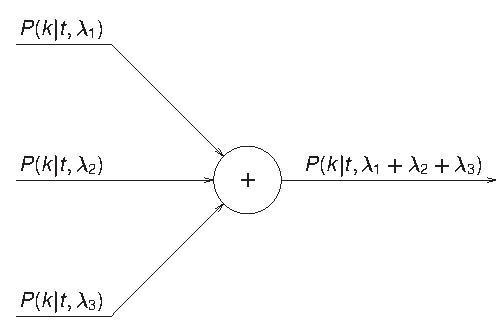
\includegraphics{diagrams/sumPoisson}
\par\end{centering}

\caption{If independent Poisson processes form a single traffic flow overall
process is a Poisson with a rate that s the sum of the rates of the
separate processes.\label{cap:poissonSuperposition}}

\end{figure}


~


\foilhead[-0.5in]{Example of Poisson Superposition}
\begin{itemize}
\item Example 1, Chapter 4


There are three queues for registration of MSc students from different
courses at the University of Sheffield. Students for the first course,
Physics and Fine Art, arrive with a rate of 4 students per minute.
Students for the second course, The Psychology of Sociology, arrive
with a rate of 2 students per minute and students for the third course,
Computer Science and Aromatherapy arrive with a rate of 5 students
a minute.

Assuming the student arrivals are independent and occur as a Poisson
process what is the probability that after 15 minutes there have been
\textbf{a)} 90 student arrivals? \textbf{b)} 180 arrivals?



\end{itemize}

\foilhead[-0.5in]{Properties Contd}
\begin{itemize}
\item Decomposition of Poisson Flow


Assume we have one input channel where arrivals are occurring with
a Poisson process with rate $\lambda$. This channel then splits into
$N$ separate output channels. Each input arrival is then independently
assigned to output channel $n$ with probability $P\left(n\right)$.
In this case the output channels then behave like Poisson processes
with rates given by $\lambda_{n}=P\left(n\right)\lambda$. This is
shown in Figure~\ref{cap:decompositionPoisson}.

\end{itemize}
%
\begin{figure}[ht]
\begin{centering}
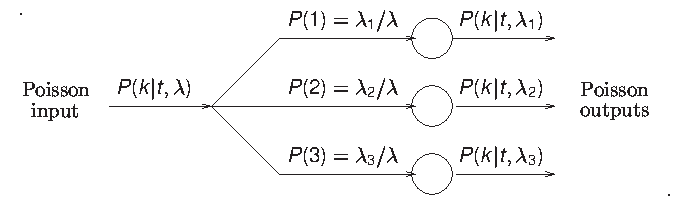
\includegraphics{diagrams/decomposePoisson}
\par\end{centering}

\caption{If a single Poisson process with rate $\lambda$ is switched to different
output channels, with each arrival being switched to channel $n$
with probability $P\left(n\right)=\lambda_{n}/\lambda$, each output
channel will be a Poisson process with rate $\lambda_{n}$.\label{cap:decompositionPoisson}}

\end{figure}


~


\foilhead[-0.5in]{Example of Poisson Decomposition}
\begin{itemize}
\item Example 2, Chapter 4


There is one registration for all MSc courses. Students arrive in
the hall and are assigned to registration desks according to the first
letter of their surname. Desk 1 ($d=1)$takes students with names
from A-G, desk 2 ($d=2$) from H-M, desk 3 ($d=3$) from N to S and
desk 4 ($d=4$) from R to Z. 

Surnames are distributed amoungst these four categories with the following
probability distribution:

\begin{center}
\begin{tabular}{|c|c|c|c|c|}
\hline 
$d$ & 1 & 2 & 3 & 4\tabularnewline
\hline
\hline 
$P\left(d\right)$ & $0.20$ & $0.27$ & $0.25$ & $0.28$\tabularnewline
\hline
\end{tabular}
\par\end{center}

Assuming the students arrive independently of their surname as a Poisson
process at a rate of 10 students per minute what is the probability
that \textbf{a)} after 5 minutes 5 students have arrived at desk 1?
\textbf{b)} after 10 minutes 20 students have arrived at desk 4?

\end{itemize}

\foilhead[-0.5in]{Properties III}
\begin{itemize}
\item Independence of Arrivals\label{sub:poissonIndependence}


Consider a single Poisson process, if we look within this process
at two \emph{disjoint} time intervals (\emph{i.e.} periods of time
that don't overlap). Assume we have $k_{1}$ arrivals in the first
interval and $k_{2}$ arrivals in the second interval. The distribution
of arrivals in the two intervals are independent of each other, $P\left(k_{1},k_{2}\right)=P\left(k_{1}\right)P\left(k_{2}\right)$. 

\end{itemize}

\foilhead[-0.5in]{Properties IV}
\begin{itemize}
\item Similarity of Arrival Distributions for Identical Intervals\label{sub:poissonSimilarities}


Consider a single Poisson process with rate $\lambda$, let the number
of arrivals between time $s$ and $s+t$ be given by $k_{1}$. Now
consider a second independent Poisson process with the same rate $\lambda$,
let the number of arrivals between time $r$ and $r+t$ be given by
$k_{2}$. The distribution of $k_{1}$ and $k_{2}$ are then equal,
\[
P\left(k_{1}\right)=P\left(k_{2}\right).\]
 

\end{itemize}

\foilhead[-0.5in]{Interarrival Times and Poisson Processes}
\begin{itemize}
\item Interarrival time: time between arrivals.
\item Think of buses.
\item $X_{i}$, are continuous values, what is their PDF?.
\end{itemize}

\foilhead[-0.5in]{Interarrival Distribution}
\begin{itemize}
\item Example 3, Chapter 4. Derivation of Interarrival Time Distribution


%
\begin{figure}[ht]
\begin{centering}
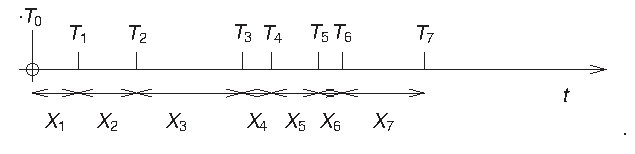
\includegraphics{diagrams/interArrivals}
\par\end{centering}

\caption{For a Poisson process, this figure shows the times of the arrivals,
$T_{n}$, and the interarrival times, $X_{n}$.\label{cap:poissonInterArrival}}

\end{figure}


In the figure above we show different arrival times $T_{1},\dots,T_{n}$
for the process. You can think of these as the arrival times of the
buses. We are interested in computing the distribution of the variables
$X_{i}=T_{i}-T_{i-1}$: the times between bus arrivals. In this example
you will derive this PDF for the interarrival times%
\footnote{The interarrival times, $X_{i}$, are continuous values, so they will
be governed by a probability density function rather than a discrete
probability distribution.%
}.



\end{itemize}

\foilhead[-0.5in]{Properties of the Exponential Distribution}
\begin{itemize}
\item The Memoryless property\[
P\left(X>s+t|X>t\right)=P\left(X>s\right)\]

\item In English, the probability of the waiting time being greater than
$s+t$ given that the waiting time is already greater than $t$ is
the same as the probability of the waiting time being greater than
$s$.
\item Mean and Variance\[
p(x)=\lambda e^{-\lambda x}\]
 


The mean of an exponential can be found to be, \[
\left\langle x\right\rangle _{p(x)}=\frac{1}{\lambda}\]
 and the variance is \[
\left\langle x^{2}\right\rangle _{p(x)}-\left\langle x\right\rangle _{p(x)}^{2}=\frac{1}{\lambda^{2}}.\]
 These are easily confirmed --- they are part of Tutorial 1. 

\end{itemize}

\foilhead[-0.5in]{Markov Chains and Markov Processes\label{cha:markovChainsAndProcesses}}

Poisson process in a special case of the more general class of processes
known as Markov processes. We will start by considering Markov processes
as they operate in \emph{discrete time}, otherwise known as \emph{Markov
chains}. Both Markov processes and Markov chains exhibit the \emph{Markov
property} which is an assumption about how future values drawn from
the process depend on past values. We will first discuss the Markov
property in the context of Markov chains, then we will show how a
discrete system can be converted to a continuous system.


\foilhead[-0.5in]{Markov Chains}
\begin{itemize}
\item Consider a discrete representation of time $t=0,1,2...$. We associate
a state variable, $N$, with this time such that we have values for
$N$ at $N(0),\, N(1),\, N(2),\,...$. 
\item Turns in a board game.
\item Markov Property

\begin{itemize}
\item value at time $t$ is dependent only on its value at time $t-1$. 
\item The future is conditional independent of the past (the conditioning
being on the present).
\item State of the system in the future is \emph{not} dependent on what
happened in the past if we know the state at the present time.
\end{itemize}
\end{itemize}

\foilhead[-0.5in]{Monopoly}
\begin{itemize}
\item A real-life example of a Markov chain
\item Forty squares on a Monopoly board. %
\begin{figure}[ht]
\begin{centering}
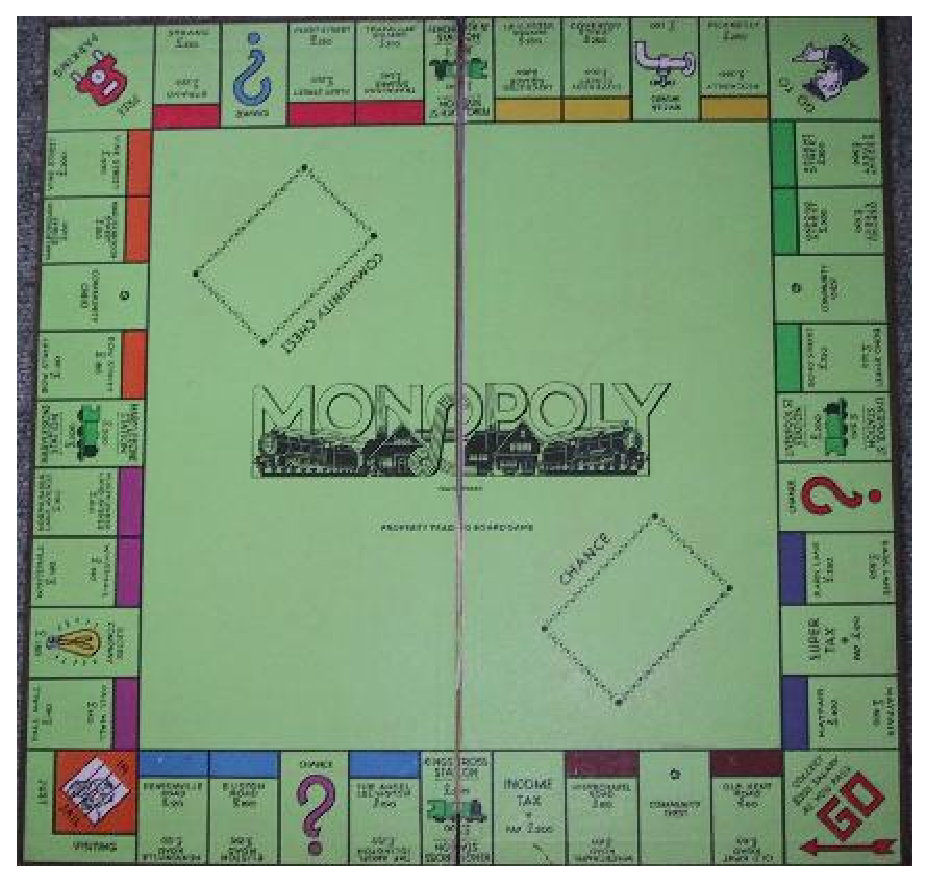
\includegraphics{diagrams/smallMonopoly}
\par\end{centering}

\caption{Image of a monopoly board.}

\end{figure}

\end{itemize}

\foilhead[-0.5in]{Markov Chain Monopoly}
\begin{itemize}
\item Player's state, $N(t)$, square number +40$\times$number of `GO's


Normally move through two six sided dice and adding them together.
Denote the result of this die roll $d(t)$. 

\item State at time $t$ is


\[
N(t)=N(t-1)+d(t).\]
 Monopoly exhibits the Markov property, future states are independent
of your previous states given your current state.

\end{itemize}

\foilhead[-0.5in]{State Diagrams}

A Markov chain can be represented by a state diagram just as finite
state machines are often represented in this manner. One important
difference is that Markov chains are not necessarily finite, they
can have infinity states! A further difference is that the transitions
for Markov chains are associated with probabilities (or in the case
of Markov processes rates).


\foilhead[-0.5in]{Poisson Process as a Markov Process}

We've introduced the game of Monopoly as a Markov chain. In this next
session we shall relate Markov chains, where time is treated as a
discrete variable, to Markov processes, where time is a continuous
variable. We will show how the Poisson process is a special case of
a Markov process where a constrained set of transitions are allowed.
To do this we will first introduce a new version of Monopoly that
we call `Coin Monopoly'. 


\foilhead[-0.5in]{Coin Monopoly}
\begin{itemize}
\item Player tosses the coin when it is their turn. 
\item We take $d(t)=0$ if a coin is tails and $d(t)=1$ if it is heads.
This is depicted as a state diagram in Figure~\ref{cap:coinMonopolyStateDiagram}. 
\end{itemize}
%
\begin{figure}[ht]
\begin{centering}
\answer{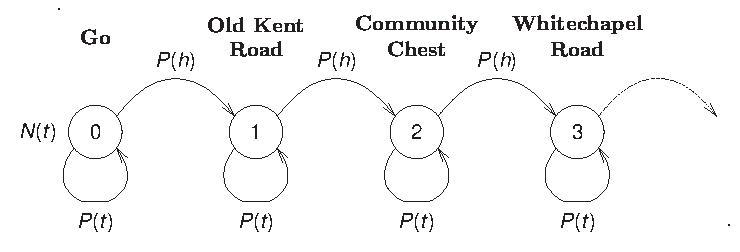
\includegraphics{diagrams/stateDiagram}}{6}
\par\end{centering}

\caption{State diagram for coin monopoly. Each node (circle) represents a different
possible state value. The state changes (or doesn't change) with each
time step according the probabilities associated with the arrows.
\label{cap:coinMonopolyStateDiagram}}

\end{figure}

\begin{itemize}
\item Takes a long time to play ... let's speed it up.
\end{itemize}

\foilhead[-0.5in]{Fast Coin Monopoly}
\begin{itemize}
\item Time, $t$, originally changes by $\Delta t=1$. 
\item Special coin with $P\left(h\right)=\lambda\,\Delta t$ (which must
be less than 1), giving $P\left(t\right)=1-\lambda\,\,\Delta t$. 
\item Use the \emph{binomial distribution} to compute how many heads.
\end{itemize}

\foilhead[-0.5in]{Binomial Distribution for $n$ Trials}
\begin{itemize}
\item Example 1, Chapter 5. It is possible to compute a probability distribution
for a number of successes given a number of trials. This distribution
is known as the binomial. For $n$ trials (equivalent to $n$ coin
tosses or $n$ turns for Coin Monopoly) the probability of $k$ successes
(equivalent to $k$ moves forward) is given by 


\begin{equation}
P\left(k\right)=\left(\begin{array}{c}
n\\
k\end{array}\right)P\left(h\right)^{k}(1-P\left(h\right))^{n-k}\label{eq:binomialDistirbution}\end{equation}
where $\left(\begin{array}{c}
n\\
k\end{array}\right)=\frac{n!}{k!(n-k)!}$ is known as the binomial coefficient. 

By considering the limiting case as the probability of a success (or
heads) goes to zero but the number of trials goes to $\infty$ show
that a Poisson process can be recovered.

\end{itemize}

\foilhead[-0.5in]{Markov Process State Diagrams}

%
\begin{figure}[ht]
\begin{centering}
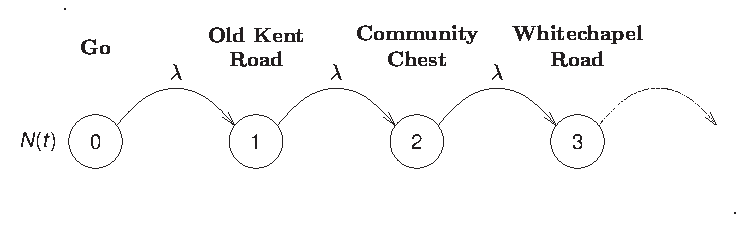
\includegraphics{diagrams/stateDiagramProcess}
\par\end{centering}

\caption{State diagram for the Markov process given by Coin Monopoly in the
limit as $\Delta t\rightarrow0$. This is the state diagram for a
Poisson process. Notice in comparison to Figure~\ref{cap:coinMonopolyStateDiagram},
the probabilities have been replaced by rates and there are no self-transition
arrows.\label{cap:coinMonopolyProcess}}

\end{figure}



\foilhead[-0.5in]{Summary}

You've now seen that a Poisson process can be derived starting from
a simple Markov chain. This gives some deeper insight to a Poisson
process. In the coin monopoly model there is a fixed (constant) probability
of moving forward in every turn and whether a move forward occurs
in each turn is completely independent of what happened in previous
turns. The Poisson process is the continuous analogue of this stem.
There is a constant probability of an arrival occurring at any time
which is independent of what has gone before. This gives you an intuitive
explanation of the two properties of the Poisson process --- similarity
and independence.


\foilhead[-0.5in]{Steady State\label{sec:steadyState}}
\begin{itemize}
\item Steady state behaviour vs the transient dynamics. 
\item What do we mean by steady state? 

\begin{enumerate}
\item A stable condition that does not change over time or in which change
in one direction is continually balanced by change in another.%
\footnote{\texttt{http://www.dictionary.com}.%
}
\item A steady state is a dynamic equilibrium. 
\end{enumerate}
\item A Markov process \emph{can} reach a steady state distribtuion. 
\end{itemize}

\foilhead[-0.5in]{Steady State contd}
\begin{itemize}
\item A probabilistic process $p\left(k|t\right)$ is a `noisy function'
of time. 

\begin{itemize}
\item If process converges to a distribution as time $\rightarrow\infty$
then it has a steady state.\[
\lim_{t\rightarrow\infty}p\left(k|t\right)=p\left(k\right)\]
the average value of $k$ at steady state is then given by\[
\left\langle k\right\rangle _{p\left(k\right)}=\sum_{k=0}^{\infty}p\left(k\right)k.\]

\end{itemize}
\item A Poisson process doesn't have a steady state distribution.
\end{itemize}

\foilhead[-0.5in]{Coin Monopoly Revisited}
\begin{itemize}
\item `Coin Monopoly' Markov chain (as we described it) has no \emph{steady
state} distribution

\begin{itemize}
\item Over time the value of $k$ will always increase. 
\end{itemize}
\item In this lecture introduce a (slightly) more complex Markov process:
the \emph{birth-death processes}. 
\item A birth-death process can have a steady state distribution. 
\item We use detailed balance to discover this distribution.
\end{itemize}

\foilhead[-0.5in]{Birth Death Process}
\begin{itemize}
\item A model for births and deaths in a population. 
\item Recall the Markov chain underlying `Coin Monopoly'. 

\begin{itemize}
\item Modify this diagram: allow backwards moves. 
\item Prevent state from going negative. 
\item This system is known as a birth-death process. 
\end{itemize}
\end{itemize}
%
\begin{figure}[ht]
\begin{centering}
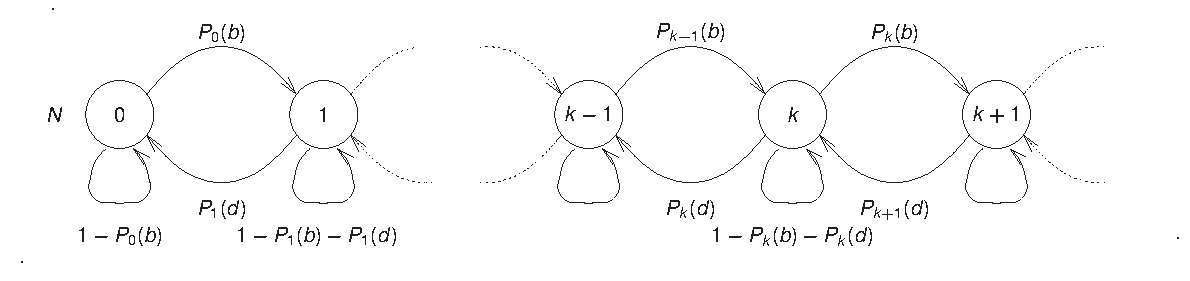
\includegraphics[width=1\textwidth]{diagrams/birthDeathChain}
\par\end{centering}

\caption{State diagram for a birth-death chain.\label{cap:birthDeathChainState}}

\end{figure}


%
\begin{figure}[ht]
\begin{centering}
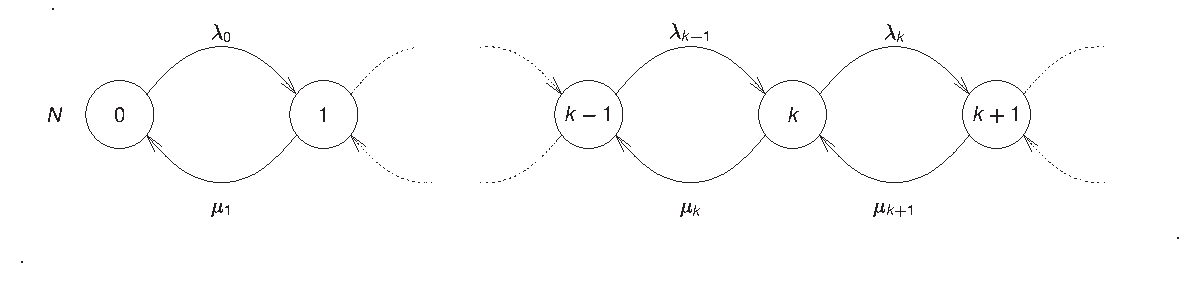
\includegraphics[width=1\textwidth]{diagrams/birthDeathProcess}
\par\end{centering}

\caption{State diagram for a birth-death process.\label{cap:birthDeathChainProcess}}

\end{figure}



\foilhead[-0.5in]{Kendall's Notation\label{sec:kendall}}
\begin{itemize}
\item Simple way of summarising the characteristics of a queue.
\end{itemize}
\begin{center}
%
\begin{minipage}[c][1\totalheight][t]{4cm}%
\begin{center}
Arrival characteristics
\par\end{center}%
\end{minipage}{\LARGE /}%
\begin{minipage}[c][1\totalheight][t]{4cm}%
\begin{center}
Departure characteristics
\par\end{center}%
\end{minipage}{\LARGE /}%
\begin{minipage}[c][1\totalheight][t]{4cm}%
\begin{center}
number of servers 
\par\end{center}%
\end{minipage}{\LARGE /}%
\begin{minipage}[c][1\totalheight][t]{4cm}%
\begin{center}
max number of customers
\par\end{center}%
\end{minipage}
\par\end{center}

The arrival and departure characteristics are summarised by
\begin{itemize}
\item $M$ --- Markov --- Poisson distributed arrivals, exponentially distributed
service times.
\item $D$ --- Deterministically distributed times.
\item $G$ --- General distribution for inter-arrival/service times.
\end{itemize}

\foilhead[-0.5in]{Global Balance}
\begin{itemize}
\item Seek a stationary distribution through global balance equations. 
\item At equilibrium the frequency of transitions out of state $k$ equals
the frequency of transitions into $k$ \cite[pg 260-262]{Bertsekas:data92}. 
\item Markov chain can be defined by a transition probability matrix.

\begin{itemize}
\item Gives the probability of transition from any state to any other. \[
\mathbf{P}=\left[\begin{array}{ccccc}
P_{11} & \cdots & P_{i1} & \cdots & P_{N1}\\
\vdots & \ddots &  &  & \vdots\\
P_{1j} &  & P_{ij} &  & P_{Nj}\\
\vdots &  &  & \ddots & \vdots\\
P_{1N} & \cdots & P_{iN} & \cdots & P_{NN}\end{array}\right].\]
where probability of transition from state $i$ to state $j$ is given
by $P_{ij}$.
\end{itemize}
\end{itemize}

\foilhead[-0.5in]{Global Balance II}
\begin{itemize}
\item If $P\left(j\right)$ is steady state probability for state $j$,
global balance says\[
P\left(j\right)\sum_{i=0}^{\infty}P_{ji}=\sum_{i=0}^{\infty}P\left(i\right)P_{ij}\]
``the probability of leaving state $j$ should be equal to the probability
of arriving in state $j$.''
\item Markov Process: rates of transfer. 
\item Rates of transfer between states are given by a matrix with elements
$q_{ij}$ for transfer between $i$ and $j$. Global balance equations
give\[
P\left(j\right)\sum_{i=0}^{\infty}q_{ji}=\sum_{i=0}^{\infty}P\left(i\right)q_{ij}.\]

\end{itemize}

\foilhead[-0.5in]{Detailed Balance}
\begin{itemize}
\item For the birth death processes transitions only between state $k$
and $k+1$ or $k-1$. 

\begin{itemize}
\item $P_{ij}=0$ if $i>j+1$ and $i<j-1$. 
\end{itemize}
\item Special case of the global balance: detailed balance equations. Looks
at the flow between two states. 
\item For the discrete case\[
P\left(k-1\right)P_{k-1,k}=P\left(k\right)P_{k,k-1}\]

\item For the continuous case \[
P\left(k-1\right)q_{k-1,k}=P\left(k\right)q_{k,k-1}.\]

\item With our notation rate from $q_{k-1,k}=\lambda_{k-1}$ and $q_{k,k-1}=\mu_{k}$
giving
\end{itemize}
\[
P\left(k-1\right)\lambda_{k-1}=P\left(k\right)\mu_{k}.\]



\foilhead[-0.5in]{Boundary Flow}
\begin{itemize}
\item Consider the flow rates at a \emph{boundary} between two states, $k-1$
and $k$. 


%
\begin{figure}[ht]
\begin{centering}
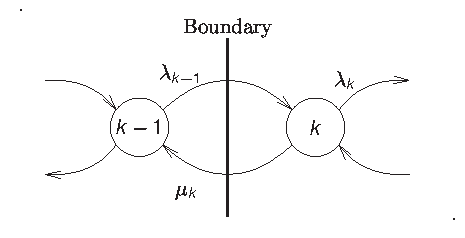
\includegraphics[width=0.6\textwidth]{diagrams/boundaryFlow}
\par\end{centering}

\caption{Flow rates at a Boundary for a birth-death process.\label{cap:flowAtBoundary}}

\end{figure}


\item At steady state

\begin{itemize}
\item flow from $k-1$ to $k$ is $\lambda_{k-1}P\left(k-1\right)$, 
\item flow from $k$ to $k-1$ is $\mu_{k}P\left(k\right)$. 
\end{itemize}
\item For flow to be balanced we have \[
\lambda_{k-1}P\left(k-1\right)=\mu_{k}P\left(k\right).\]
 
\item For different systems birth rate and death rate will differ. First
we consider $M/M/1$ queue.
\end{itemize}

\foilhead[-0.5in]{Kendall's Notation --- $M/M/1$}

\begin{center}
%
\begin{minipage}[c][1\totalheight][t]{4cm}%
\begin{center}
Arrival characteristics
\par\end{center}%
\end{minipage}{\LARGE /}%
\begin{minipage}[c][1\totalheight][t]{4cm}%
\begin{center}
Departure characteristics
\par\end{center}%
\end{minipage}{\LARGE /}%
\begin{minipage}[c][1\totalheight][t]{4cm}%
\begin{center}
number of servers 
\par\end{center}%
\end{minipage}{\LARGE /}%
\begin{minipage}[c][1\totalheight][t]{4cm}%
\begin{center}
max number of customers
\par\end{center}%
\end{minipage}
\par\end{center}

\begin{center}
{\Large $M/M/1$}
\par\end{center}{\Large \par}
\begin{itemize}
\item \textcolor{red}{\large $M$ --- Markov --- Poisson distributed arrivals,
exponentially distributed service times.}{\large \par}
\item \textcolor{cyan}{$D$ --- Deterministically distributed times.}
\item \textcolor{cyan}{$G$ --- General distribution for inter-arrival/service
times.}
\end{itemize}

\foilhead[-0.5in]{$M/M/1$ Queue\label{sec:MM1Stationary}}
\begin{itemize}
\item $M/M/1$ arrivals occur as a Poisson process, service times are exponentially
distributed. 
\item A birth-death process

\begin{itemize}
\item constant birth rate $\lambda_{k}=\lambda$ (from the Poisson process) 
\item constant death rate (from the exponentially distributed service times)
$\mu_{k}=\mu$. 
\end{itemize}
\item State diagram is 
\end{itemize}
{\tiny }%
\begin{figure}[ht]
\begin{centering}
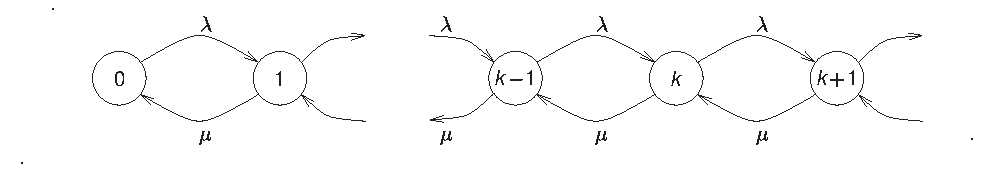
\includegraphics[width=1\textwidth]{diagrams/stateMM1}
\par\end{centering}

\caption{State diagram for $M/M/1$ queue. }

\end{figure}
{\tiny \par}
\begin{itemize}
\item Derive stationary distribution is derived using detailed balance. 
\end{itemize}

\foilhead[-0.5in]{$M/M/1$ Stationary Distribution}
\begin{itemize}
\item The state diagram highlights several points. 

\begin{enumerate}
\item There are no transitions to a state below 0.
\item There is no maximum value for the state shown, this implies that $k$
is unbounded.
\item The birth rates and death rates for each state are indicated. 
\item Transitions are only possible between neighbouring states.
\end{enumerate}
\item Flow at boundary: analyse between $k$ and $k-1$.


%
\begin{figure}[ht]
\begin{centering}
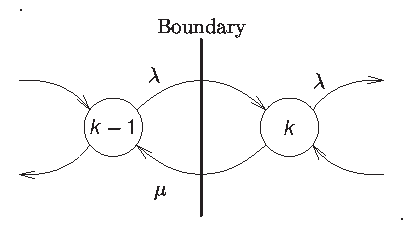
\includegraphics[width=0.6\textwidth]{diagrams/boundaryFlowMM1}
\par\end{centering}

\caption{Flow rates at a boundary.\label{cap:flowAtBoundary}}

\end{figure}


\item At steady state, \[
\lambda P\left(k-1\right)=\mu P\left(k\right).\]
 
\end{itemize}

\foilhead[-0.5in]{$M/M/1$ --- Stationary Distribution II}
\begin{itemize}
\item At steady state, \[
\lambda P\left(k-1\right)=\mu P\left(k\right).\]
 
\item Leading to \[
P\left(k\right)=\frac{\lambda}{\mu}P\left(k-1\right).\]
 
\item Thus\begin{eqnarray*}
P\left(k\right) & = & \left(\frac{\lambda}{\mu}\right)^{k}P\left(0\right)\\
 & = & \rho^{k}P\left(0\right),\end{eqnarray*}
 


where we have defined $\rho=\frac{\lambda}{\mu}$, which, for the
$M/M/1$ queue, is called the \emph{utilisation factor}. 

\end{itemize}

\foilhead[-0.5in]{Normalisation\label{sub:normalisationMM1}}
\begin{itemize}
\item To find $P\left(0\right)$ we use the normalisation condition.\[
\sum_{k=0}^{\infty}P\left(k\right)=1\]
 and because $P\left(k\right)=\rho^{k}P\left(0\right)$,\[
1=P\left(0\right)\sum_{k=0}^{\infty}\rho^{k}\]
 giving \begin{equation}
P\left(0\right)=\frac{1}{\sum_{k=0}^{\infty}\rho^{k}}.\label{eq:MM1Series}\end{equation}
 
\item The infinite series in the denominator converges if $\rho<1$ (when
$\lambda<\mu$), \[
\sum_{k=0}^{\infty}\rho^{k}=\frac{1}{1-\rho}\,\,\,\textrm{for\,\,\,\ensuremath{\rho<1}},\]
 so $P\left(0\right)=\left(1-\rho\right)$ and the full distribution
for the \emph{steady state} probabilities is \[
P\left(k\right)=\rho^{k}\left(1-\rho\right).\]

\end{itemize}

\foilhead[-0.5in]{Faster Arrivals than Service}

Notice that if the arrival rate (birth rate) is greater than the service
rate (death rate) then $\rho>1$ and the series in (\ref{eq:MM1Series})
doesn't converge. This is indicative of the fact that if the birth
rate is greater than the death rate there is no steady state distribution.
The queue continues to grow in size.


\foilhead[-0.5in]{Average Number in System}
\begin{itemize}
\item Network design: interested in the average queue length. 
\item We use the steady state probabilities to compute this quantity. 
\item The average number of customers in the system \emph{is not} the same
as the average queue length 

\begin{itemize}
\item a customer being served (\emph{e.g.} a packet under transmission)
is not in the queue.
\end{itemize}
\item Average number of customers in the system is the expected state of
the system.
\end{itemize}
\[
\left\langle k\right\rangle _{P\left(k\right)}=\sum_{k=0}^{\infty}kP\left(k\right)\]



\foilhead[-0.5in]{Average Number in System II}

Example 1, Chapter 6. The average number in the system for the $M/M/1$
queue is given by considering the steady state distribution. Compute
this value.

The variance is computed as an excercise in the Tutorial Sheet.

\[
\textrm{var}\left[k\right]=\left\langle k^{2}\right\rangle -\left\langle k\right\rangle ^{2}=\frac{\rho}{\left(1-\rho\right)^{2}}.\]
 


\foilhead[-0.5in]{Discrete Simulation of $M/M/1$}
\begin{itemize}
\item Next week: first lab class.
\item Discrete simulation of an $M/M/1$ queue: easy to run because it takes
the form of a Markov chain. 
\item State diagram for this system.


%
\begin{figure}[ht]
\begin{centering}
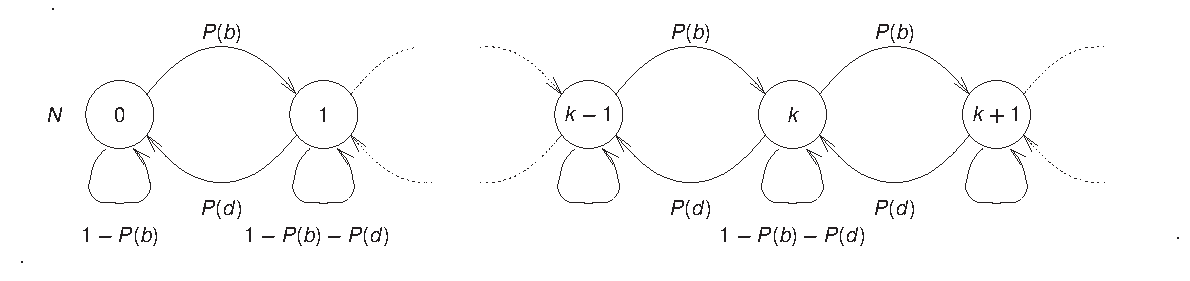
\includegraphics[width=1\textwidth]{diagrams/discreteMM1State}
\par\end{centering}

\caption{State diagram for the discrete version of the $M/M/1$ queue.}

\end{figure}


\end{itemize}

\foilhead[-0.5in]{Hints for the Simulation}
\begin{itemize}
\item Use a loop over discrete time steps. 
\item At each time step there are three possible events: 

\begin{itemize}
\item the state of the system increases by one; 
\item the state of the system decreases by one and 
\item the state of the system stays the same. 
\end{itemize}
\item Modelling the queue is therefore a simple matter of testing which
of these outcomes is true. 


%
\begin{figure}[ht]
\begin{centering}
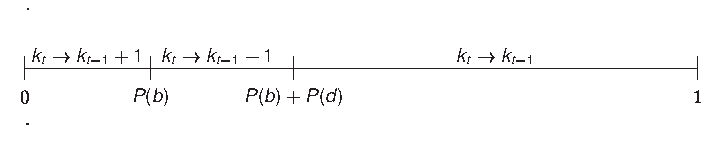
\includegraphics[width=0.8\textwidth]{diagrams/probOutcome}
\par\end{centering}

\caption{Testing for one of three outcomes. Generate a random number and see
where it lands.}

\end{figure}


\end{itemize}

\foilhead[-0.5in]{Approximating a Continuous $M/M/1$ Queue}
\begin{itemize}
\item We know from last week that a Poisson process can be derived by considering
the limit of a simple Markov chain. 
\item A continuous $M/M/1$ queue is the limit of the discrete model we
are using for simulation
\item In your lab class you can make ths approximation by taking $\Delta t$
to be much smaller than $\lambda$ or $\mu$. 
\item Then you may set $P\left(b\right)=\lambda\Delta t$ and $P\left(d\right)=\mu\Delta t$. 
\end{itemize}

\foilhead[-0.5in]{Demonstration}
\begin{itemize}
\item Lab class: run a simulation of the discrete queue.
\item Answer questions on the analysis of that queue. 
\item Now we demonstrate a simulation in the lecture. 
\item We also give you histograms that are similar to those you should be
producing in the lab class.
\end{itemize}

\foilhead[-0.5in]{Histograms}

%
\begin{figure*}[ht]
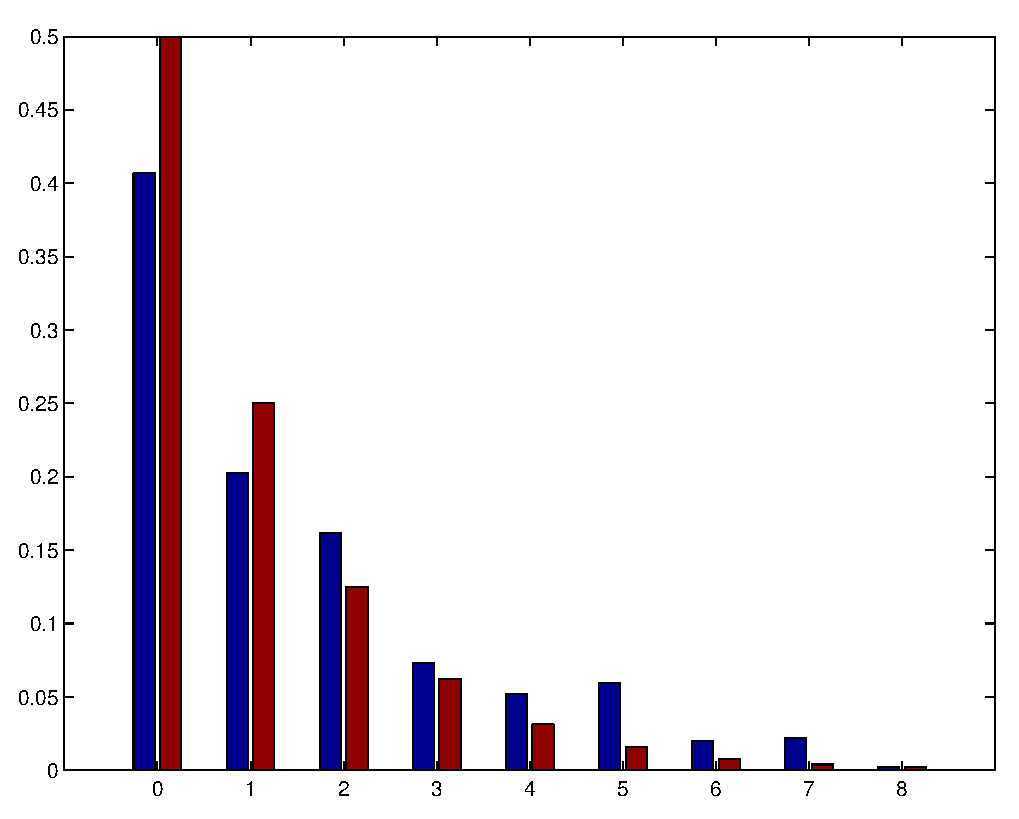
\includegraphics[width=0.45\textwidth]{diagrams/rho_half_100_arrivals}
\hfill{}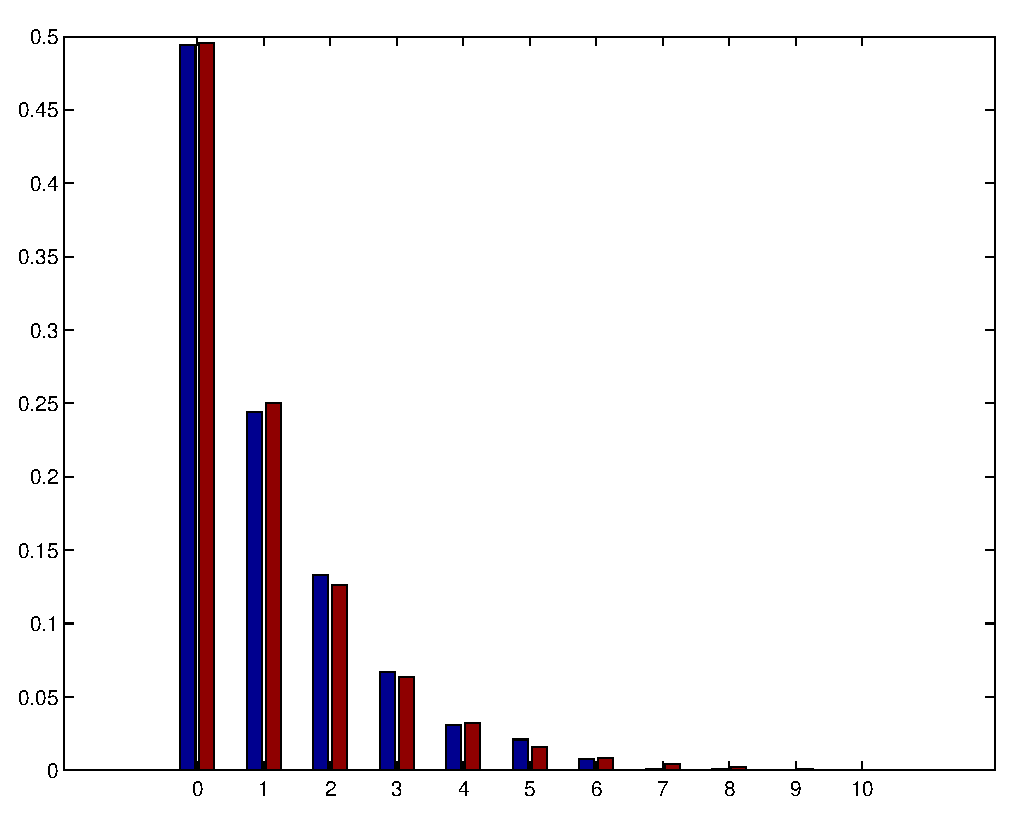
\includegraphics[width=0.45\textwidth]{diagrams/rho_half_1000_arrivals}

\caption{Left figure: steady state probabilities after the first 100 seconds
for $\rho=0.5$. Right figure: steady state probabilities after the
first 1000 seconds for $\rho=0.5$.}

\end{figure*}


%
\begin{figure*}[ht]
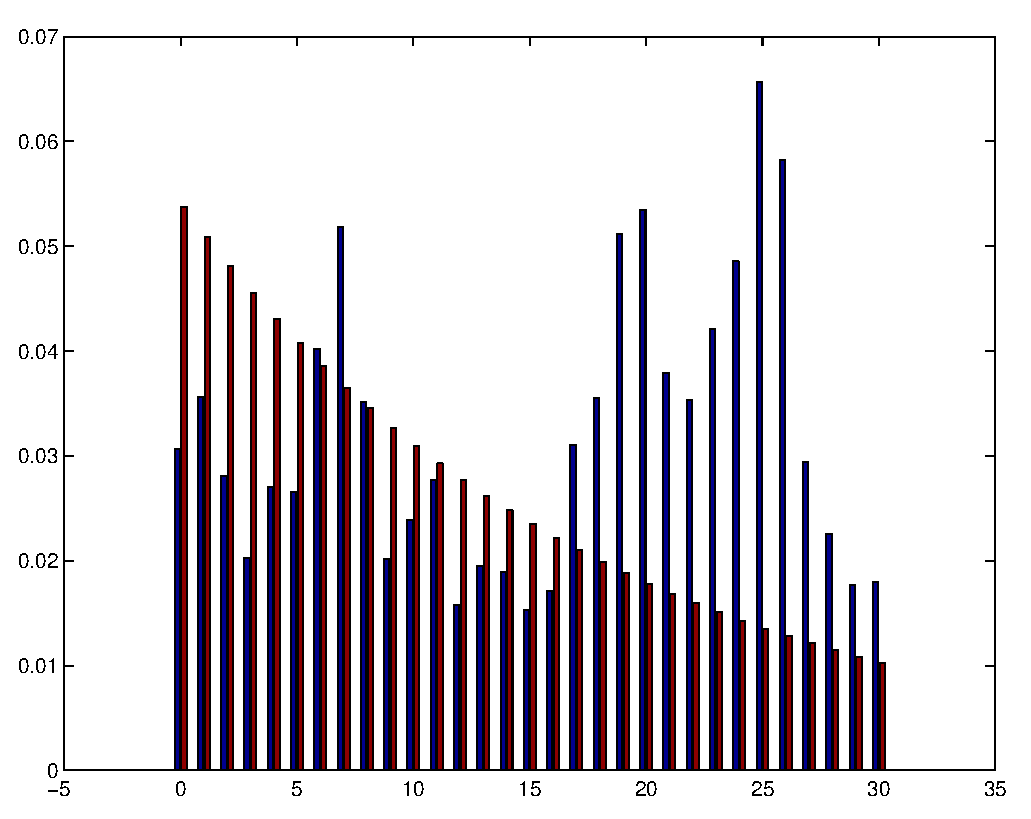
\includegraphics[width=0.45\textwidth]{diagrams/rho_point95_100_arrivals}
\hfill{}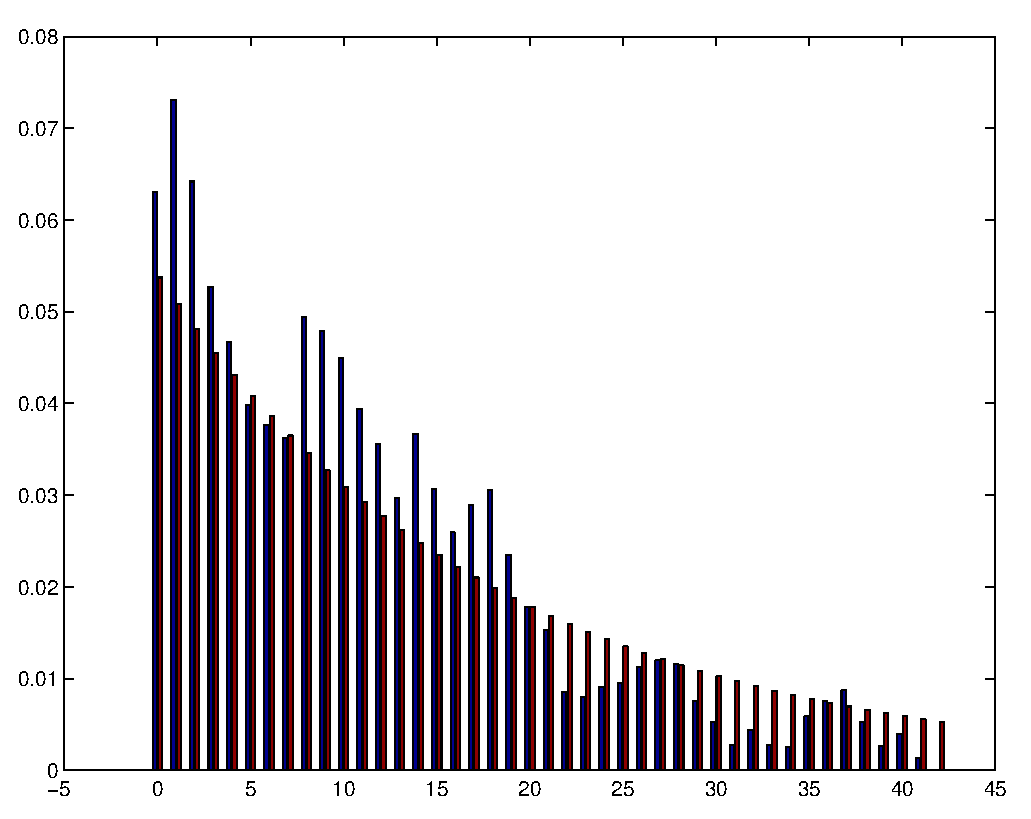
\includegraphics[width=0.45\textwidth]{diagrams/rho_point95_1000_arrivals}

\caption{Left figure: steady state probabilities after the first 100 seconds
for $\rho=0.95$. Right figure: steady state probabilities after the
first 1000 seconds for $\rho=0.95$.}

\end{figure*}



\foilhead[-0.5in]{Little's Formula}
\begin{itemize}
\item Important quality of service issue is the average delay.
\item We would also like to be able to compute 

\begin{itemize}
\item the average number in the queue and 
\item the average time spent queueing.
\end{itemize}
\item We introduce Little's formula, a very general formula.
\item Can be applied to $G/G/1$ queues. 
\item Gives the relationship between 

\begin{itemize}
\item Steady-state average size of a queue, $\bar{N}$. 
\item The steady-state arrival rate, $\lambda$.
\item The steady-state customer delay, $\bar{T}$. 
\end{itemize}
\end{itemize}

\foilhead[-0.5in]{Time and Steady State Averages}
\begin{itemize}
\item We have already introduced the distribution means and sample based
means. 
\item Time based averages are a further type of average. 
\item The time average is the average value of a particular function over
time.\[
\bar{f}_{t}=\frac{1}{t}\int_{0}^{t}f\left(\tau\right)d\tau.\]

\item The derivation of Little's formula relies on an assumption. 

\begin{itemize}
\item Assume that averages under the steady state distribution are equivalent
to the time average in the limit as $t\rightarrow\infty$, 
\item Average number in the system as a function of time is given by \[
\bar{N}_{t}=\frac{1}{t}\int_{0}^{t}N\left(\tau\right)d\tau\]
and the time average after in the limit as $t\rightarrow\infty$ is
given by \[
\bar{N}=\lim_{t\rightarrow\infty}\bar{N}\left(t\right).\]
which we assume is equivalent to $\left\langle k\right\rangle _{p\left(k\right)}\equiv\bar{N}$.
See pg 156-157 in \cite{Bertsekas:data92}. 
\end{itemize}
\end{itemize}

\foilhead[-0.5in]{The Formula}
\begin{itemize}
\item Applies under steady state conditions.
\item Under the steady state assumptions it states,\[
\bar{N}=\lambda\bar{T}.\]

\end{itemize}
\textbf{Example}: Nightclub queue.

You are driving past a nightclub, wondering how long you will have
to wait to go in. You notice on Thursday nights that the queue typically
contains 20 people and that people arrive at a rate of 40 per hour. 

According to Little's formula, how long would you expect to have to
wait to get in? 

\textbf{Answer}

\answer{The waiting time is given by Little's formula: 

$\bar{N}=20$, $\lambda=40$ and $\bar{T}=\frac{\bar{N}}{\lambda}=\frac{20}{40}=\frac{1}{2}\textrm{hour}$.
}{6}


\foilhead[-0.5in]{Intuition}

If we see there are twenty people in a queue and they enter a building
at a rate of 40 per hour, we might expect to have to wait half-an-hour
in the queue. Formally though, we will build upon the intuition with
a simple graphical `proof' of the formula based upon that given in
\cite{Bertsekas:data92}.


\foilhead[-0.5in]{Graphical Proof I}

Example 1, Chapter 7. Graphical Proff of Little's Formula.


\foilhead[-0.5in]{Little's Formula}

\[
\bar{N}=\lambda\bar{T}\]

\begin{itemize}
\item Applies regardless of the arrival and service time distributions.
\item Relies on the system being in \emph{steady state}. 
\item Can be used at the level of the system.
\item Or the level of the queue.
\item Or the level of service.
\end{itemize}

\foilhead[-0.5in]{Average Delay in $M/M/1$}
\begin{itemize}
\item The mean of the steady state distribution for an $M/M/1$ queue is\[
\bar{N}=\frac{\lambda}{\mu-\lambda}=\frac{\rho}{1-\rho}.\]

\item Can use Little's formula to tell us the average delay.
\item From $\bar{N}=\lambda\bar{T}$ we rearrange to recover \[
\bar{T}=\frac{1}{\mu-\lambda}\]
 
\item This is not the time spent in the queue! 
\item This is the time spent in the system: it includes \emph{service time.}

\begin{itemize}
\item arises from \emph{propagation delay.}
\item length of phone call \emph{etc}.
\end{itemize}
\end{itemize}

\foilhead[-0.5in]{Little's Formula for Queueing Time and Transmission Time }
\begin{itemize}
\item The total delay can be divided into 

\begin{itemize}
\item queueing time, $W$, 
\item and service time $X$. \[
T=X+W.\]
 
\end{itemize}
\item Similarly the average delay may be decomposed as\[
\bar{T}=\bar{X}+\bar{W}.\]
 
\item The queue and transmission may the be analysed independently using
Little's formula.
\end{itemize}

\foilhead[-0.5in]{The Transmission}
\begin{itemize}
\item Assume that customers/packets do not leave the queue. 
\item Rate of arrivals at the queue must equal the rate of arrivals at transmission. 
\item We define the the average number under transmission as $\rho$ \[
\rho=\lambda\bar{X},\]
where $\bar{X}$ is the average time spend under transmission for
each packet. 
\item For the $M/M/1$ queue the average transmission time is given by $\bar{X}=\frac{1}{\mu}$, 
\item So for the $M/M/1$ queue we have\[
\rho=\frac{\lambda}{\mu},\]
 a formula which we have already used in the last chapter. 
\end{itemize}

\foilhead[-0.5in]{Utilisation Factor}
\begin{itemize}
\item $\rho$ is the utilisation factor. 
\item Represents the fraction of time that the transmission line (or server)
is in use.
\item It is a measure of efficiency. 
\item It is also the steady state probability that the transmission line
is in use. 
\item For a lossless system this probability is given by $1-P\left(0\right)$. 
\end{itemize}

\foilhead[-0.5in]{Utilisation Example}

Example 2, Chapter 7. Simple example of Little's formula. You are
at a queue in a bar and notice that the bar tender spends 10\% of
her time cleaning between customers. If the typical number of people
waiting to be served is 3 what is the ratio of time spent serving
to time being served?


\foilhead[-0.5in]{The Queue}
\begin{itemize}
\item For arrival rate $\lambda$, and $\bar{N}_{Q}$, the average number
in queue, and $\bar{W}$, the average queueing (waiting) time.\[
\bar{N}_{Q}=\lambda\bar{W}\]

\item For the $M/M/1$ queue \[
\bar{T}=\bar{X}+\bar{W}=\frac{1}{\mu}+\bar{W}\]
 so the average time spent waiting in the queue is given by\[
\bar{W}=\bar{T}-\frac{1}{\mu}=\frac{\rho}{\mu-\lambda}.\]

\item Average number in the queue is then\[
\bar{N}_{Q}=\frac{\rho^{2}}{1-\rho}.\]
 
\end{itemize}

\foilhead[-0.5in]{References}

\bibliographystyle{abbrv}
\bibliography{lawrence,other,zbooks}


\end{document}
